\documentclass[a4paper,11pt]{book}
\renewcommand{\familydefault}{\sfdefault}

\usepackage{standalone}
\usepackage[english]{babel}
\usepackage[top=3cm]{geometry}
\usepackage{float}
\usepackage{tabularx}
\usepackage{multirow}
\usepackage{booktabs}
\usepackage{pgfplots}
\usepackage{amsmath}
\usepackage{amssymb}
\usepackage{amsfonts}
\usepackage{siunitx}
\usepackage{tikz}
\usepackage{graphics} % for pdf, bitmapped graphics files
\usepackage{graphicx}
\usepackage{exsheets}
\usepackage{algorithm}
\usepackage{algorithmicx}
\usepackage[noend]{algpseudocode}
\usepackage{hyperref}
\usepackage{enumitem}
\usepackage{filecontents}
\usepackage{multirow}
%\usepackage{showframe}% to show frames
%\ifCLASSOPTIONcompsoc
\usepackage[caption=false, font=normalsize, labelfont=sf, textfont=sf]{subfig}
%\else
%\usepackage[caption=false, font=footnotesize]{subfig}
%\fi    

\usetikzlibrary{patterns,arrows,arrows.meta,calc,intersections,shapes,positioning,decorations.pathreplacing,decorations.markings,decorations.pathmorphing}
\usepackage{multicol}

\sisetup{output-decimal-marker={,},exponent-product=\cdot}

\DeclareSIUnit\atm{atm}
\DeclareSIUnit\dioptre{D}



\def\BState{\State\hskip-\ALG@thistlm}


\definecolor{TitleColor}{rgb}{0.65,0.04,0.07}
\definecolor{NumberColor}{rgb}{0.02,0.04,0.48}

\DeclareInstance{exsheets-heading}{fancy}{default}{
toc-reversed = true ,
indent-first = true ,
vscale = 2 ,
pre-code = \IfInsideQuestionT{\rule{\linewidth}{1pt}} ,
post-code =\IfInsideQuestionT{\rule{\linewidth}{1pt}} ,
subtitle-format = \large\scshape\color{rgb:red,0.65;green,0.04;blue,0.07} ,
number-format = \large\bfseries\color{rgb:red,0.02;green,0.04;blue,0.48} ,
points-format = \itshape ,
join = { number[r,B]title[l,B](.333em,0pt);
title[r,B]subtitle[l,B](1em,0pt)
} ,
attach =
{
main[hc,vc]number[hc,vc](0pt,0pt) ;
main[l,vc]subtitle[hc,vc](\marginparsep,0pt)
}
}



\DeclareInstance{exsheets-heading}{block-subtitle}{default}{
vscale = 2 ,
pre-code = \rule{\linewidth}{1pt} ,
post-code = \rule{\linewidth}{1pt} ,%title-format = \large\scshape\color{TitleColor} ,
number-format = \large\bfseries\color{rgb:red,0.02;green,0.04;blue,0.48} ,
subtitle-format = \large\scshape\color{black} ,
join = {
title[r,B]number[l,B](.333em,0pt) ;
title[r,B]subtitle[l,B](1em,0pt)
} ,
attach = {
main[l,vc]title[l,vc](0pt,0pt) ;
main[r,vc]points[l,vc](\marginparsep,0pt)
},
}

\DeclareQuestionClass{textbook}{textbooks}

\SetupExSheets{
  headings = fancy,
  question/print = true ,
  solution/print = false }
 % counter-format = se.qu ,
%  counter-within = section ,
  %question/pre-hook = \rule{\textwidth}{1pt},


\hypersetup{
	colorlinks = true, 
	breaklinks = true, 
	bookmarks = true,
	bookmarksnumbered = true,
	urlcolor = blue, 
	linkcolor = blue, 
	citecolor=blue,
	linktoc=page, 
	pdftitle={}, 
	pdfauthor={\textcopyright Author}, 
	pdfsubject={}, 
	pdfkeywords={}, 
	pdfcreator={pdfLaTeX}, % PDF Creator
	pdfproducer={IEEE} }





\tikzset{point/.style={circle,fill,black!80,inner sep=0pt,minimum size=#1,opacity=0.9}}
\tikzset{point/.default=3pt}\tikzset{vector/.style={line width=1pt,postaction={decorate,decoration={markings,mark=at position 1 with {\arrow{latex}}}}}}
\tikzset{block/.style={rectangle,fill=black!30,draw,minimum size=#1,opacity=0.9,align=center}}
\tikzset{block/.default=15pt}\tikzset{ball/.style={circle,fill=black!30,draw,minimum size=#1,opacity=0.9}}
\tikzset{ball/.default=5pt}\tikzset{pulley/.style={draw=black,line width=0.2pt,circle,minimum size=#1,inner sep=0pt,fill=black!10}}
\tikzset{pulley/.default=20pt}\tikzset{rod/.style={line width=2pt}}
\tikzset{rope/.style={line width=1pt}}
\tikzset{spring/.style={decorate,decoration={coil,amplitude=5pt,segment length=#1,aspect=0.3}}}
\tikzset{spring/.default=5pt}\tikzset{wall/.style={black!10,pattern=north east lines,opacity=0.3}}
\tikzset{ray/.style={line width=0.8pt,postaction={decorate,decoration={markings,mark=at position 0.5 with {\arrow{>}}}}}}
\tikzset{arrow/.style={-latex}}
\tikzset{object/.style={line width=1pt,orange,-latex}}
\tikzset{image/.style={line width=1pt,blue,-latex}}
\tikzset{doublearrow/.style={<->,>=latex,thick}}
\tikzset{brace/.style={decorate,decoration={brace,amplitude=#1}}}
\tikzset{brace/.default=5pt}




\graphicspath{{images/}} 




\makeatletter
\@addtoreset{question}{section}
\makeatother


\begin{document}
\author{Dr. Muhammed Rushdi \and Asem Alaa}

\title{Measurements and Instrumentation [SBE206A] (Fall 2018)\\ Tutorial 7}

\maketitle


\chapter*{Errors during the measurement process}

\section*{Introduction}
\begin{itemize}
\item Measurement errors are impossible to avoid.
\item we can minimize their magnitude by: 
\begin{itemize}
\item good measurement system design.
\item appropriate analysis and processing of measurement data.
\end{itemize} 
\item Errors are categorized to:
\begin{itemize}
\item Systematic errors
\item Random errors
\end{itemize}
\end{itemize}

\section*{Systematic errors}

The systematic errors affect the readings in a consistent way, such that all readings are on one side of the true value (either all positive or all negative).\\
\\
Sources of systematic errors are:
\begin{enumerate}
\item System disturbances due to measurement.
\item Environmental changes (results in change of sensitivity drift or zero drift).
\item Use of uncalibrated instruments.
\item Wear in instruments components (can be compensated by calibration).
\item Poor cabling practices.
\end{enumerate}






\section*{Random errors}

In contrast, random errors have stochastic effects on readings; the readings are distributed around a the true value.  \\ \\  
Possible sources of random errors are:
\begin{enumerate}
\item Human reading errors.
\item Electrical noise.
\end{enumerate}

\section*{Comparison between systematic and random errors}
\begin{figure*}[h!]\label{fig:uncertinity}
\centering
  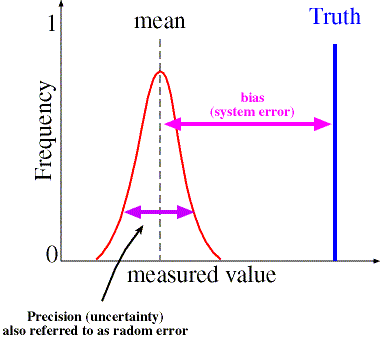
\includegraphics[width=0.8\linewidth]{uncertinity}
  \caption{Difference between systematic errors effect and random errors effect.} 
\end{figure*}

\begin{table}
\begin{tabular}{|c|c|}
\hline 
Systematic Error & Random Error \\ 
\hline 
Poor accuracy & poor precision \\ 
\hline 
definite causes & indefinite causes \\ 
\hline 
reproducible & not reproducible \\ 
\hline 
\end{tabular} 
\caption{Comparison between systematic and random errors}
\end{table}

\begin{question}
Which is more challenging? Systematic errors or random errors?
\end{question}
\begin{solution}


\end{solution}


\section*{Aggregation of measurement system errors}

\chapter*{Problems}

\section*{Systematic Errors}
\subsection*{Systematic erros due to disturbance}
\begin{question}[subtitle=System Disturbance]
\begin{figure*}[h!]\label{fig:systematic_error_circuit}
\centering
  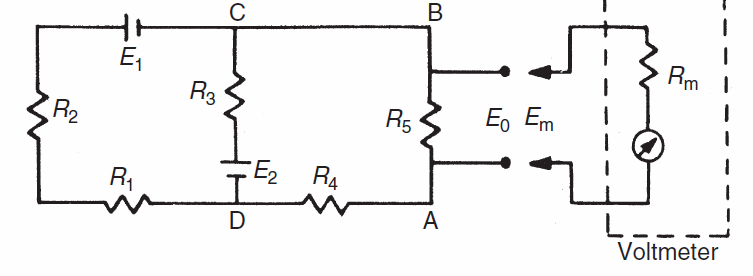
\includegraphics[width=0.8\linewidth]{systematic_error_circuit}
  \caption{Effect of applying the voltmeter to the measured quantity.} 
\end{figure*}
\begin{enumerate}
\item Derive the relation of the true and output readings.
\item Suppose that the components of the circuit in Figure \ref{fig:systematic_error_circuit} have the following values:
 R\textsubscript{1} = $400\Omega$, R\textsubscript{2} = $600\Omega$, R\textsubscript{3} = $1000\Omega$, R\textsubscript{4} = $500\Omega$, R\textsubscript{5} = $1000\Omega$
\end{enumerate}
\examspace*{10em}

\end{question}
\begin{solution}


\end{solution}


\begin{question}


\examspace*{10em}

\end{question}
\begin{solution}


\end{solution}






\end{document}
